%----------------------------------------------------------------------------------------
%	CHAPTER 2
%----------------------------------------------------------------------------------------

\chapter{Background}\label{Background}

This chapter will provide the reader with background knowledge on fundamental concepts in this thesis.\\

This chapter will identify and discuss the main problem with narrowband satellite link performance in more detail. Section 2.1 briefly describes the TCP protocol. Section 2.1.1 defines an Internet protocol. Section 2.1.2 takes an in-depth look at the TCP/IP protocol which is the predominant protocol used on the Internet today. Section 2.2 looks at the TCP traffic control methods which are key factors in our satellite link problem. Section 2.2.1 starts with a traffic control method as utilised from the receivers side. This TCP traffic control method is known as \emph{TCP flow control} and is key to understanding the \emph{future work} section. Section 2.2.2 presents the TCP traffic control method as utilised from the sender's side. This method is called \emph{TCP congestion control}, and this section will examine a specific component of this traffic control method most pertinent to the PEP in this thesis known as \emph{slow start}. Section 2.2.3 looks at congestion control in the satellite link environment and explains why slow start does not efficiently operate here and in fact, compounds and contributes to the problem. Section 2.2.4 takes a look at Pacific Island Internet data rates today and finally Section 2.2.5 looks at other concepts used in this thesis and provides links and references to these topics.

\section{TCP- Transmission Control Protocol}\label{TCP}
Since even before the inception of the Internet, many methods/processes and protocols have been devised to enable smooth communication between computers.  TCP/IP emerged as the fundamental communication suite in Internet communication today ~\cite{1}~\cite{2}.\\

\subsection{What is an internet protocol?}
A protocol establishes the rules of engagement between two communicating entities on the Internet. Much like humans have our protocols for proper communication to one another (e.g., taking turns speaking and listening, not talking over one another), computer networks have contracts/rules of engagement that are for the establishment of smooth communication. Many protocols have emerged since the Internet was born, but TCP/IP has become the dominant one used today ~\cite{1}~\cite{2}.

\subsection{TCP/IP protocol suite}\label{TCP/IP}
There are seven layers in the OSI model with TCP sitting in the higher layer referred to as the "Transport Layer" and the lower IP layer located in the "Network Layer" ~\cite{2}. For now, we will not delve much further into an explanation on the OSI layers (This will be referred to again in Section 2.2.5) as we will keep our focus on TCP/IP in general terms for now. \\

In elementary terms, we can imagine computer communication over a network as one computer passing messages or data to another computer via a complex Internet network consisting of routers and switches, other gateway computers etc. An analogy can be drawn to a person in place of a computer, sending mail in place of data or a message, via the mail system which consists of post offices and delivery via couriers over a network of highways/air routes ~\cite{1}~\cite{2}. \\

\begin{itemize}
\item TCP, the "Transmission Control Protocol" operates at the transport layer level as mentioned earlier. Regarding the analogy with the mail service, the name of the layer level itself should make it obvious that TCP would operate on the transportation of the mail ~\cite{2}. TCP encompasses the overall transportation and safe, reliable delivery of packages/mail/letters from their starting point to their final target destination. Such a mail service would include:\\
\begin{enumerate}
\item Ways of keeping track of the package as it is shipped via the highway (sequence numbers in TCP) between sender and receiver.
\item Policies in place to ensure mail centres or delivery trucks are not overloaded with packages. A means of controlling the flow of packages through the mail system in an orderly fashion (congestion control).
\item A way of acknowledging reception of a package or loss of a package such as the signature requirements in a parcel delivery (ACKs) ~\cite{1}~\cite{2}.\\
\end{enumerate}

\item TCP concepts include \emph{sequence numbers} to keep track and order of the segments at the endpoints. The concept of \emph{congestion control} is also used in TCP to do as its name suggests: control congestion on the link. TCP also has its own way of acknowledging segments received utilising ACK segments. These are ways of keeping in line with the policies discussed above in the mail service ~\cite{1}.\\

\item TCP is a "connection oriented protocol" which means that a connection between two endpoints/computers in the network must be established before the transfer of data/packets can occur. TCP does this by way of a "three-way handshake" between the two endpoints. One host sends a SYN packet to initiate the connection with the target host. The target host replies with a SYN + ACK to acknowledge the request. Finally, the host responds with an ACK to accept the target host's response, and this completes the connection establishment via the three-way handshake. Data transfer between the two hosts can now begin ~\cite{1}. See diagram \ref{3way} below for more detail on how this is done ~\cite{1}~\cite{2}.  \\

\item TCP then takes the data it is meant to transmit from the higher layers in the OSI stack and breaks it into segments to be transmitted. These segments will be received by the target host whose TCP layer will then reassemble the segments into the original bytestream ~\cite{1}~\cite{2}. \\

\item TCP ensures reliability and integrity of the message meaning that it has mechanisms to ensure that the intended target host receives the message (Reliability-see Figure 2.2) and that the receiving end gets the message in its entirety without corruption (Integrity). The first part of the reliability component is the establishment of a connection between two endpoints via the three-way handshake described previously. TCP also has a sequential numbering system for every byte traversing the connection so that each data transfer/communication can be reassembled in the correct order and intact when the receiver gets it. The TCP layer at the receiver end will reassemble the data segment and deliver it up to its application layer ~\cite{1}~\cite{2}.\\

In the mail analogy, this would be akin to sending several parcels to the same address. Each parcel is numbered in a particular order (example: package 4/15), so it can be checked and assembled at its final destination (target host). The receiver of the packages can check whether all packages have been delivered using the sequence numbers. Integrity in the network sense is the inclusion of a checksum in the segment to ensure that the data has not been corrupted in any way along the route to its final destination ~\cite{1}~\cite{2}.  \\

\item IP, the Internet Protocol located in the network layer manages the end to end aspect of the communication to ensure delivery to the correct destination. In other words, IP manages the delivery of the packet to the correct target host via the destination address in the IP header of the packet. As it traverses the network, the gateway computers/routers read this address and forward it to the next gateway/router en route to the final address destination. In the postal analogy, the IP address is likened to the delivery mailing address written on the package. There may be several postal stops along the way to the final destination who will read the mailing address and forward it accordingly so that it reaches its final destination ~\cite{1}~\cite{2}. (It should be noted that the postal stops do not usually open the parcels/mail but rather just forward them on. The PEP in this thesis will be opening the parcels to view the contents). \\


\item In keeping with this analogy, we could say that different mail packages destined for the same address may take different routes depending on traffic congestion, flight availability and other such factors, but eventually they should all reach the ultimate destination. Thus this holds true for the Internet also, as individual packets may be routed differently according to the shortest path algorithms along the way. Factors such as, but not limited to, network congestion or availability of routers also impact the route chosen for each packet. Through IP, the packets will end up at the final destination eventually where they will be reassembled into the original form ~\cite{1}~\cite{2}. With Pacific Islands dependent solely on narrowband satellite link connections, however, the satellite link is always part of the path from communicating sender hosts A to target host B. The satellite link is a predictable and inevitable pathway from host A to host B in the TCP connection. Hence, conventional shortest path algorithms have little, to no influence on improving segment round trip times (RTT). This is especially true in the Pacific island region where any terrestrial latency on the island would be negligible due to the small land mass ~\cite{4}~\cite{5}.

\end{itemize}

\begin{figure}[h]
    \centering
    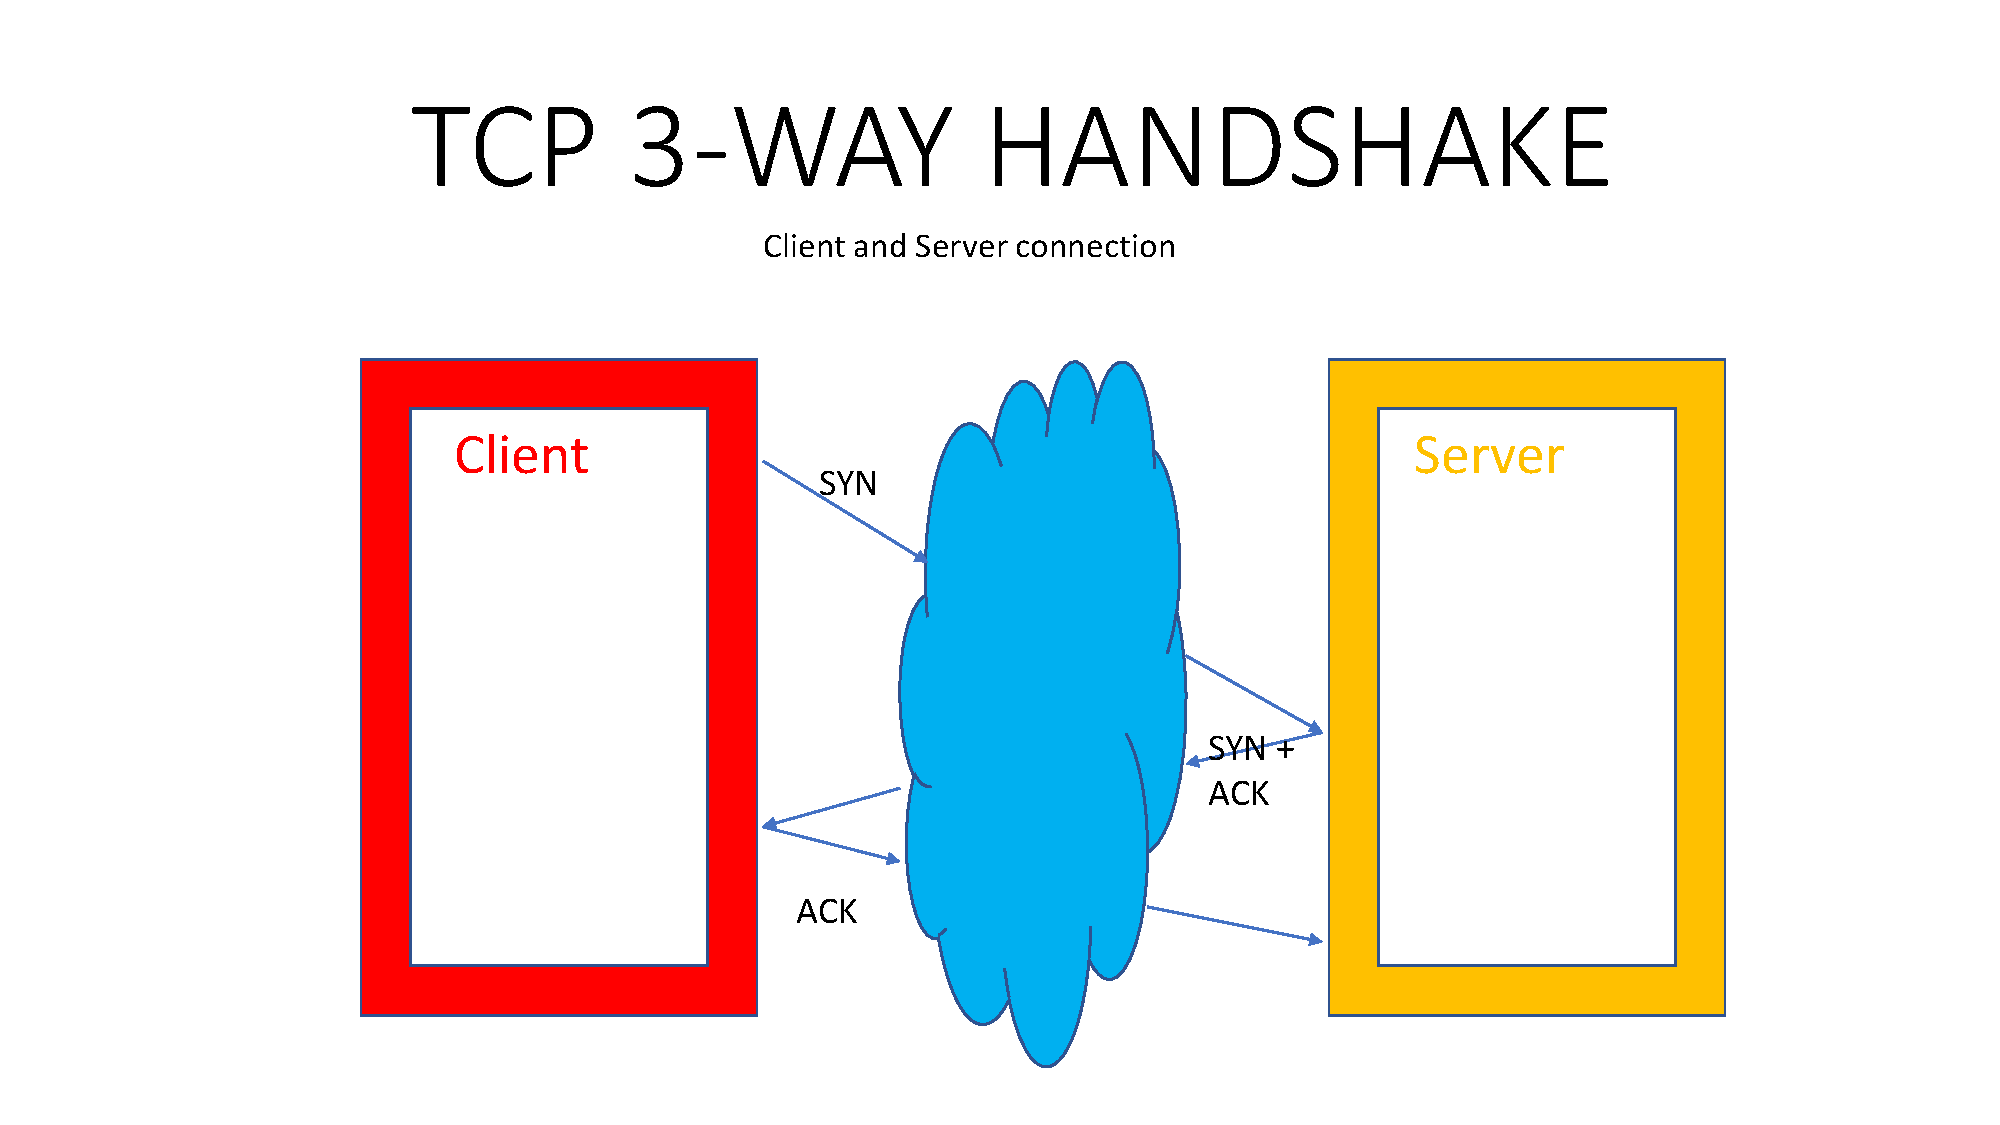
\includegraphics[width=1.0\textwidth]{3way.pdf}
    \caption{TCP three-way handshake. }
    \label{3way}
\end{figure}


\begin{figure}[h]
    \centering
    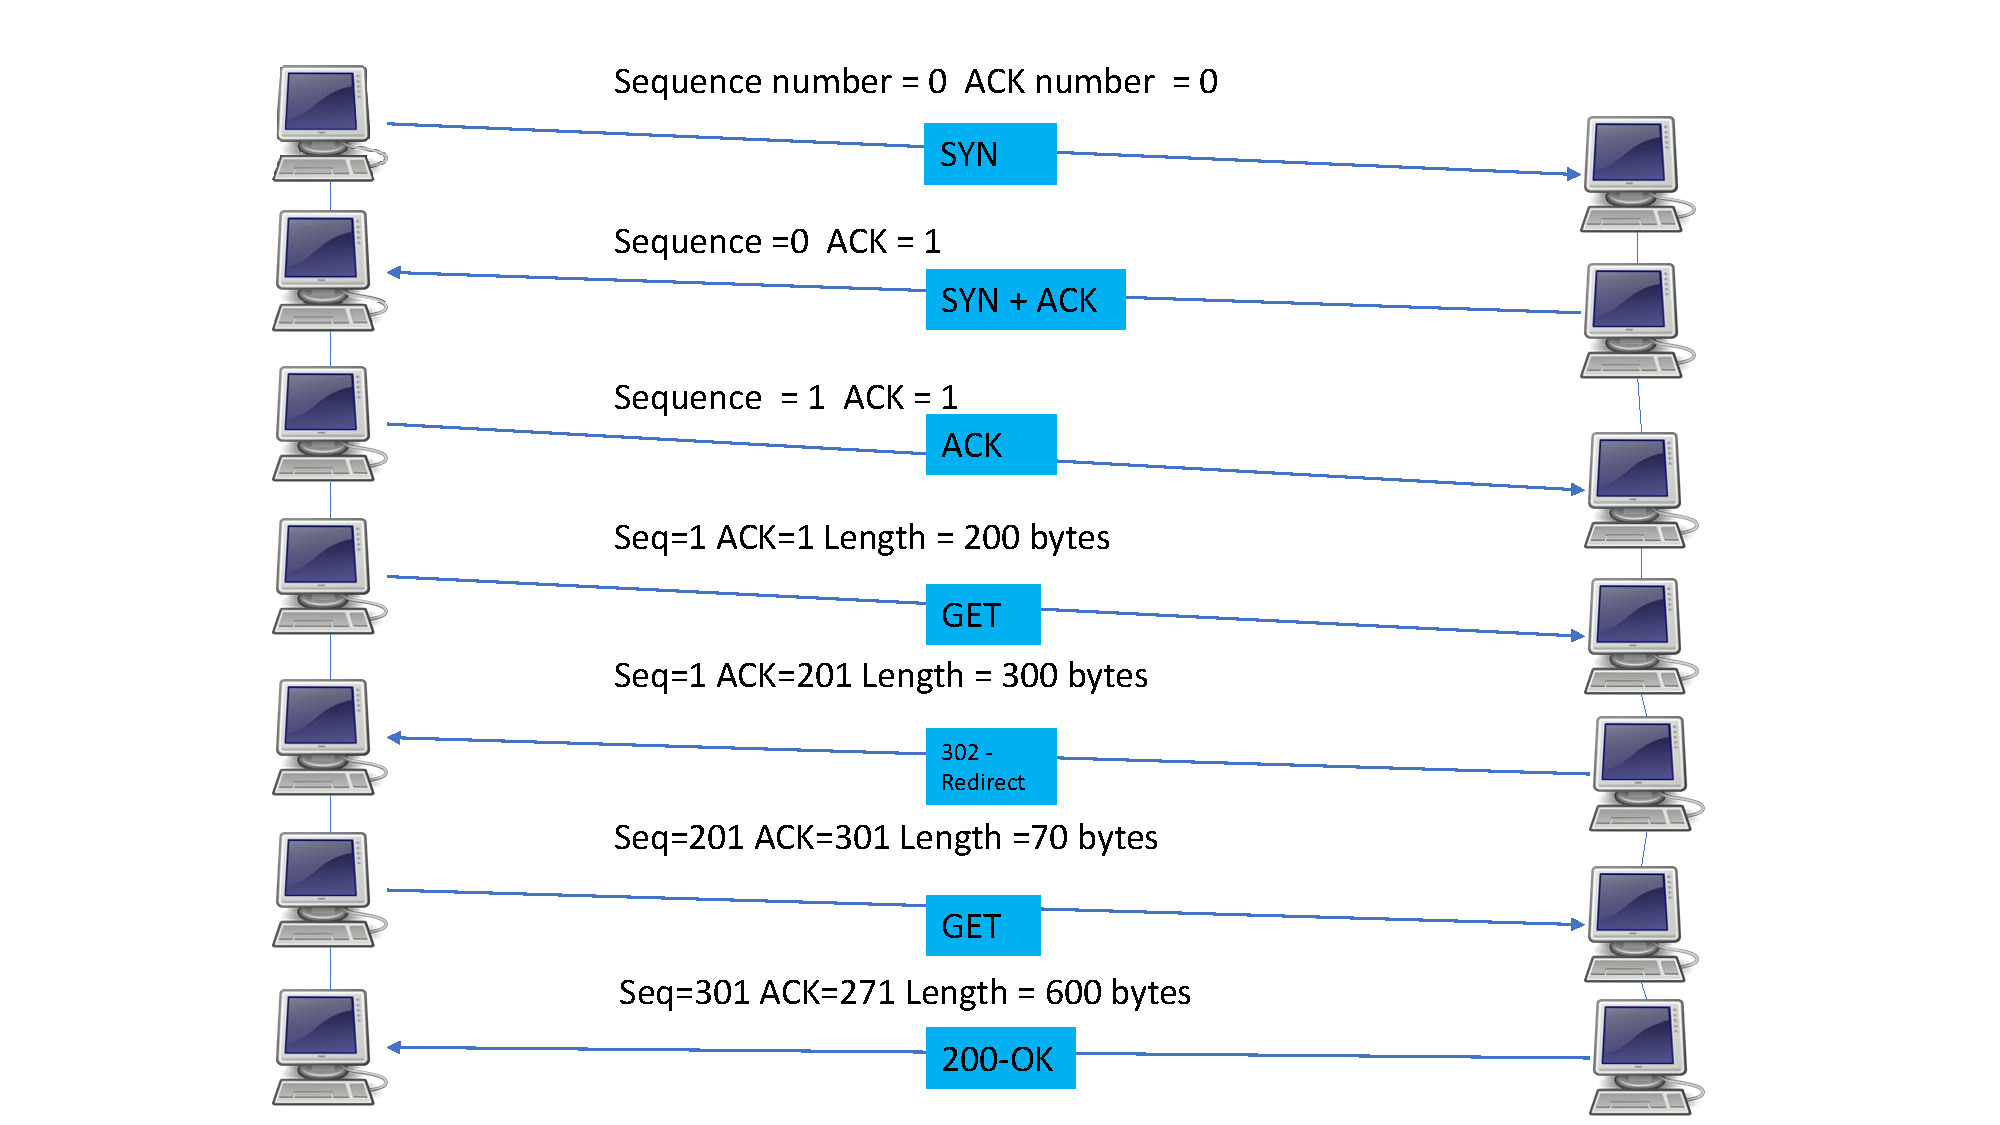
\includegraphics[width=1.1\textwidth]{ACK.pdf}
    \caption{Reliable Data Transport}
    \label{Reliable}
\end{figure}

\section{TCP Traffic Control Methods}\label{TCP Traffic Control}
Now that we have been given a brief overview of TCP and how it works, let us look into the aspect of TCP that relates to the main problem we are examining in this thesis, namely that of latency in narrowband satellite links. 

\subsection{TCP flow control}\label{TCP Flow Control}
TCP Flow control was invented in 1988 by Van Jacobson in response to the Internet's first ever congestion collapse in 1986 on a link from LBL to UC Berkeley ~\cite{19}. This collapse was caused by the sender sending packets to the receiver faster than the receiver can process them which results in the receiver being overwhelmed and collapsing under the weight of transmission ~\cite{19}. \\

Since then, many forms of TCP flow control have been implemented. TCP flow control, in basic terms, is a way for the receiver of data to communicate to the sender and control the amount of data they send so that they do not get overloaded. TCP flow control is now mandatory on all TCP Connections ~\cite{1}. to mitigate these problems. It performs this function via a sliding window mechanism that enables the adjustment of the data rate retransmission dependent on the destinations \emph{receive window}. The target has a certain amount of bytes that it can store in a TCP buffer space. If the amount of data received exceeds the TCP store buffer space, the result is packet loss which is an undesirable outcome ~\cite{1}~\cite{19}.. \\


As the number of bytes in the destination's TCP buffer space accumulate, they will eventually be transferred up for processing to the Application Layer. This clears some of the TCP buffer space for arrival of new packets. TCP Flow control is used to control data flow in the event the receiver is bombarded with data too quickly. Ideally the arrival rate of new packets should match or be slightly less than the rate at which the application layer programs read and clear data from the buffer for processing ~\cite{2}~\cite{19}.\\

The destination host can let the sender know the amount of available buffer space via the form of an advertised window in an ACK back to the sender. The advertised window or receiver window (rwnd) will be read by the sender so that it does not send any data exceeding the advertised amount of bytes in the next exchange. (If the destination host should get wholly overwhelmed, it will advertise a zero byte window, and this will tell the sender to back off completely. The sender will send \emph{keep alive} packets in response to keep the connection open until the receiver recovers and can free up TCP buffer space again) ~\cite{1}~\cite{2}~\cite{19}. \\

It is analogous to filling a bucket with water if it has a hole in it. If water is poured into the bucket too quickly, it will not drain in time and will eventually spill over. If the water flow is at a steady pace that allows it to drain off enough water to not overflow but also not ever be empty, then we have the desired equilibrium we want. We are using the bucket to its maximum capacity and therefore efficiently ~\cite{1}~\cite{2}\cite{19}. \\

Flow control works on the principle that a fast sender should not overwhelm a slow receiver ~\cite{1}~\cite{19}. This principle, however, is a problem that we do not generally encounter with the narrowband satellite link environment in the Pacific. Most of these satellites have bandwidths that preclude a modern day computers TCP/IP stack from being overloaded with incoming data ~\cite{4}~\cite{5}. In the case of high frequency satellites, which are not commonly used across the Pacific, flow control may become useful as the satellites are able to deliver data to earthbound hosts at GB rates ~\cite{5}. \\

TCP flow control is mentioned here, however, as it will be important in future work development for the PEP (See future work section) where modifications to the receiver window can eventually be made by the PEP to adjust for congestion on the network.

\subsection{TCP slow start/ congestion control}
TCP Slow Start is one of the congestion control mechanisms used by TCP, and it is one we will be dealing with mostly in this thesis as it relates directly to the satellite link problem we aim to resolve. Slow start slightly differs from the TCP flow control from the previous section. TCP flow control prevented the sender from overwhelming the receiver via the advertised window informing the sender of the number of bytes remaining in its buffer. \\

As stated in RFC2001 and RFC5681, old TCPs can make a connection between sender and receiver while the sender injects multiple segments into the network as per the advertised window from the receiver (flow control). This flow control mechanism works well when the sender and receiver are on the same LAN or if the data rate flow is almost identical along the path between them. Problems occur, however, when there are routers and slower links between sender and receiver. An intermediary router would then have to queue packets, and the queue itself is then at risk of being overwhelmed under massive traffic flows ~\cite{17}~\cite{18}. So congestion control deals with intermediate routers along the way that could get flooded and not the receiver (as in flow control). The intermediate routers are more likely to suffer congestion first as they typically carry multiple TCP connection flows and handle more traffic than the receiving hosts ~\cite{18}.\\

\subsubsection*{Reason the satellite link environment needs congestion control}
In the narrowband satellite situation, we have this mismatch of these link rates, as mentioned in the RFCs above, between the senders and receivers. The satellite link is a natural long latency bottleneck that will cause a queueing of packets at the input to the satellite, and it is possible for this buffer queue to be overloaded and run out of space. The bottleneck is caused by the satellites limited transmission rate (bits per second) in comparison to the terrestrial transmission rates feeding into it. The transmission rate is determined by the link's available bandwidth divided by the link's capacity ~\cite{4}~\cite{8}. There are several factors contributing to the creation of the satellites natural bottleneck situation:\\

\begin{itemize}
\item Limited availability of spectrum ~\cite{8}.
\item Limited power of the satellite ~\cite{8}.
\item Signal path loss between satellite and ground. Geostationary satellites have a very high orbit. As a result, it is very expensive to launch them that high. Economic restrictions ~\cite{8}.
\item Distance between satellite and ground ~\cite{8}.
\item Need to keep antenna size manageable ~\cite{8}.
\end{itemize}.
\\

\subsubsection*{Slow Start congestion window (cwnd)}
Slow start is a mechanism designed to mitigate the effects of congestion on a network by keeping either side, receiver or sender, from overwhelming the underlying network ~\cite{17}. We have seen the concept of a receiver window in flow control for receiver congestion (rwnd). Slow start congestion control introduces a congestion window for network congestion (cwnd). TCP uses flow control on both windows to regulate their respective traffic flows. See Figure \ref{cwnd}. \\

\begin{itemize}
\item cwnd: congestion window
\item rwnd: receiver window
\end{itemize}.
\\

As stated in the RFC 3135, the congestion window (cwnd) can be thought of as flow control enforced by the sender whereas the advertised window (rwnd) or receive window is flow control applied by the receiver ~\cite{6}. The congestion window (cwnd) is what we deal with in slow start and congestion control. The sender's evaluation of congestion in the network determines the size of the cwnd. The receiver window (rwnd) is determined by the receiver's amount of available buffer space in the TCP flow connection and is what we discussed in the TCP Flow Control section. The cwnd is maintained by the sender and is the number of packets or bytes that the sender is willing to entrust to the channel without having received ACKs for previous segments ~\cite{17}. \\

The slow start algorithm controls the rate of new packets injected by the sender into the network based on the rate of ACKs received back from the destination end. The slow start mechanism works via the implementation of congestion control at the sender. It has two parameters for this purpose, one being the cwnd (congestion window) and the ssthresh (slow start threshold) which is set to typically 10 packets in current versions of Linux ~\cite{17}~\cite{18}. \\

\begin{enumerate}
\item Congestion Window(cwnd; Initial value is 10 packets)
\item Threshhold Value(ssthresh; 65536 bytes but varies in different systems)
\end{enumerate}.
\\

When a connection between two endpoints is established via the three-way handshake, the congestion window(cwnd) is initialised to one segment of size and waits for an ACK (Acknowledgement). Note that an ACK will tell the sender how many bytes the receiver can accommodate via its advertised window and what sequence number of byte it expects next. TCP calculates the round trip time (RTT) for a sent packet A based on the arrival its corresponding ACK. TCP applies this new RTT to transmitted packet B and typically uses double the newly calculated RTT time as a timer for when it expects to receive the corresponding ACK for packet B. If the sender does not receive an ACK for the said packet B in the expected timeframe, or the sender gets a duplicate ACK from a previously sent packet A ( that is indicating it is still awaiting packet B's sequence number next), TCP will assume that packet B has been lost and retransmit it from cache for sender B ~\cite{1}~\cite{2}~\cite{17}. \\

As per the name, TCP starts slowly by sending a small number of segments initially. When it receives the corresponding ACKs back, it grows its congestion window by using the particular algorithm's growth function. Let us assume for this example that our TCP stack uses an exponential growth algorithm. (These growth algorithms differ between TCP types. E.g. TCP Reno, TCP Tahoe, Cubic etc.) ~\cite{14}~\cite{17}.  If TCP receives ACKs for these initially sent segments, it will double its cwnd which doubles the number of transmitted segments. It will repeat this process of exponentially increasing its cwnd and thus doubling segments sent out each time the sender receives the corresponding ACKs back ~\cite{17}.\\

The cwnd will continue to grow until the sender fails to receive an ACK back during the timeout period, which is an indication to the sender that a packet has been lost, possibly due to its cwnd growing too large and causing congestion. This loss tells the sender to cut back on the number of packets it is currently sending. The sender thus initiates exponential backoff and halves the size of its cwnd window. If it fails to receive another packet, it halves the size again and so forth until it has received all its ACKs. During this time it retransmits packets that are lost ~\cite{17}~\cite{18}.
See Fig 2.4.
\\
\begin{figure}[h]
    \centering
    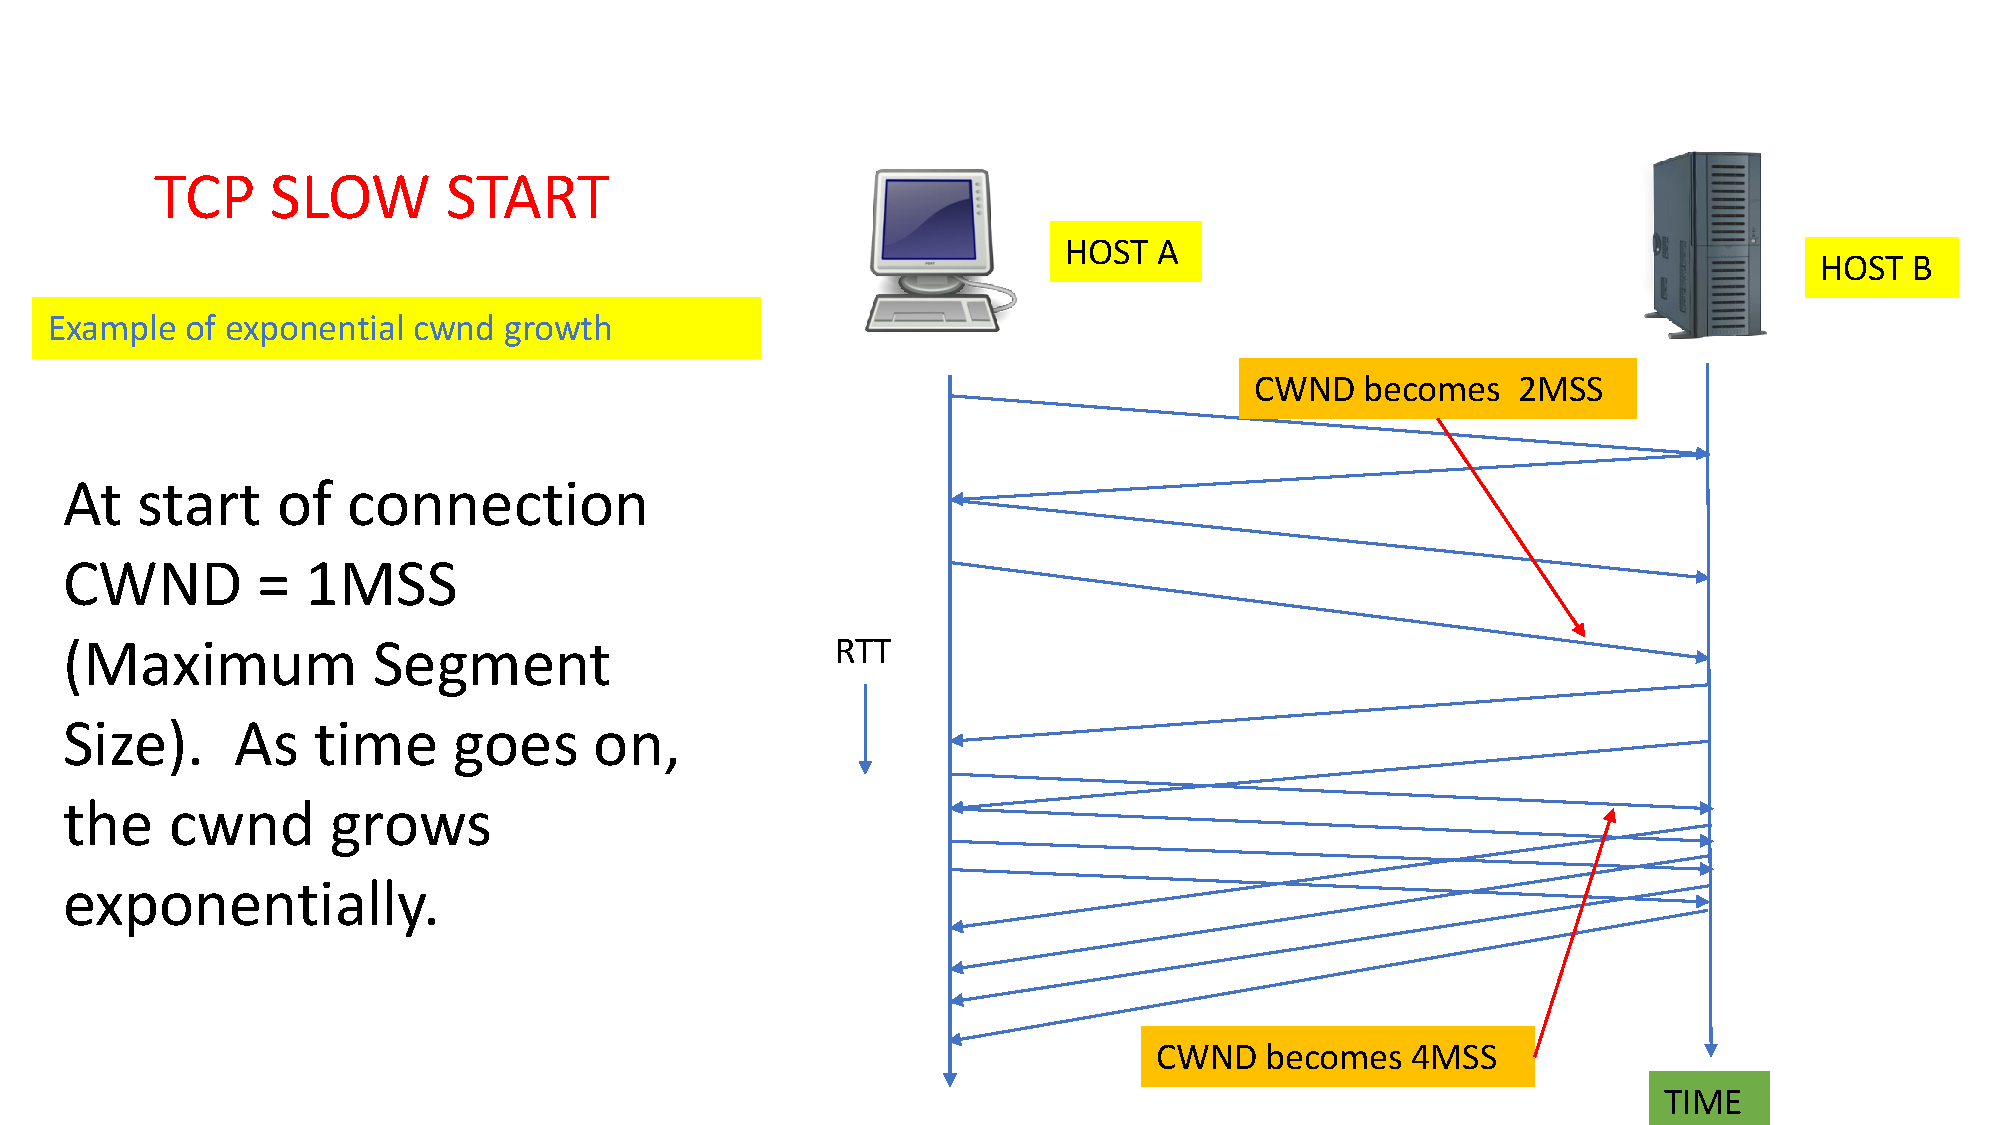
\includegraphics[width=1.0\textwidth]{tcpSlowStart.pdf}
    \caption{Example of exponential tcp slow start}
    \label{cwnd}
\end{figure}.
\\

As seen in Figure 2.5, you can visually see the exponential growth of the cwnd as each ACK comes back and it should increase to the maximum rate (bytes/RTT) allowable by the network as time passes. In a long TCP flow, we have an alternating exchange between exponential growth of cwnd and exponential backoff which should eventually stabilise once the slow start algorithm has settled upon the correct equilibrium for the congestion window. Ideally, this is how the slow start algorithm should work to mitigate against Internet network congestion ~\cite{1}~\cite{17}~\cite{18}, but it does not work so well with satellite link environments ~\cite{14}. In fact, slow start actually compounds the problem of high latency propagation delay with narrowband satellite links because it slows down the growth of the congestion window ~\cite{13}~\cite{14}. \\

\subsection{Slow Start in a satellite link environment}
Slow start becomes an issue in satellite links due to latency caused by the distance the packets must travel as outlined earlier in Section 1.1 "Problem and Motivation" and the bottleneck nature of the satellite link ~\cite{13}. The resultant "queue oscillation" as explained in more detail earlier, is caused by the combination of \emph{slow start}, the latency and the bottleneck network links ~\cite{4}~\cite{5}. \\

In a satellite link environment, the problems we have with slow start are the following; \\

\begin{enumerate}
\item The inherent latency in the link causes ACKs to arrive back to the sender much later (typically 500ms RTT in Pacific Islands). This means that even if there is no congestion on the link, slow starts cwnd in this environment grows more slowly than a typical terrestrial based TCP cwnd. The first time our senders in Pacific region, for example, can grow their cwnd is after 500ms or slightly longer depending on how far the host is from the satellite link ~\cite{4}~\cite{8}. \\
\item As the congestion window has been increased, ACKs may be returning even while the queue is overflowing because these are ACKs pertaining to packets that got through the satellite link before the queue flooded. The sender receives the ACKs believing its cwnd is too small and so TCP increases the cwnd sending more packets to an already overflowing queue. The latency in the link means that the sender will not learn about the overflowing queue for another 500ms, or longer depending on the TCP variants tolerance to lost packets. During this time, the sender will drop a large percentage of sent packets ~\cite{4}~\cite{8}.\\
\item For these lost packets, the sender will get ACK timeouts which will trigger exponential backoff. The sheer volume of packets lost due to the late discovery of the queue overflow will result in a radical decrease in sender output. Every lost ACK results in a halving of the congestion window so the sender output volume decreases rapidly until almost nothing is being outputted ~\cite{4}~\cite{8}.\\
\item  In the satellite environment, there is synchronisation between TCP senders that does not exist in the terrestrial TCP landscape.In a normal earthbound router, there are TCP flows with a mix of latencies traversing across it with different hosts receiving their ACKs at different times. Hosts in a normal network would not all ramp up their output( via slow start) or  back off at the same time. Hosts connected in a satellite link, however, all back off and ramp up simultaneously as they all receive the same outdated idea of what is happening at the satellite input queue ~\cite{4}~\cite{8}.\\
\end{enumerate}

These factors compound and perpetuate the extreme "queue oscillation" problem mentioned earlier in section 1.1. The pattern of perpetual oscillation and sawtooth patterns in network transmissions is generally of an acceptable level ~\cite{5}. In a normal terrestrial network, we have relatively low latency so the sender can get information back on dropped packets/congestion sooner and can, therefore, readjust their cwnd very quickly to suit the network conditions ~\cite{1}.\\

TCP in a typical environment can also increase the cwnd much faster as they receive the ACKs quickly due to low latency. The regular queue oscillation would occur almost entirely within its queue buffer. An overflowing and an empty buffers would be very shortlived, and filling of the buffer would be relatively slow, so packet loss is minimal ~\cite{1}~\cite{2}. If we were to print out the oscillation sawtooth pattern for a host in a standard network on an A4 sheet of paper, we would see a patterned sawtooth picture with several teeth per second running across the page. The peaks would represent the slow start cwnd ramping up very quickly, and the valleys represent the back off which also happens quickly ~\cite{1}~\cite{2}. \\

However, in narrowband satellite link transmissions, we are concerned with the extreme depth of the sawtooth pattern because the excessive burst packet losses can cause extreme backoff from all connected hosts at the same time resulting in severe link underutilisation ~\cite{4}~\cite{5}. The hosts then all ramp up again at the same time, growing their cwnd simultaneously.The satellite line queues fill quickly due to the combined influx of packets from all connected hosts ramping up simultaneously, thus repeating the cycle. If we were to print out the oscillation sawtooth pattern for a host in a satellite network across the same A4 paper, we would see a sawtooth pattern comprised of maybe one or two teeth per second with extremely high peaks representing a slow climb to grow its cwnd to a maximum. We would also see equally low valleys representing the rapid descent from exponential back off. This extreme queue oscillation and the subsequent inefficient usage of the link is a common problem with narrowband satellite links and is the main problem that this thesis aims to resolve ~\cite{4}~\cite{5}~\cite{8}.\\

So in summary, we have a bottleneck narrowband satellite link that is continuously facing two issues. Firstly, packets are continually being queued at the sender end due to the bottleneck nature of the link. The satellite link's latency means that ACKs get back too late to the sender. This lateness can cause problems 1 and 2 listed above whereby excessive sender backoff starves the the satellite uplink queue as all the senders stop emitting packets altogether for a period of time. This is an inefficient use of the link, and it is caused directly by the slow start backoff algorithm ~\cite{5}~\cite{15}. \\

Secondly, we have the issue of the cwnd window of all the senders ramping up in unison as they receive a multitude of ACKs that had been expected but assumed dropped and been retransmitted. The connected hosts all begin growing their cwnd at the same time which fills the bottleneck link queues up quickly and subsequently leads to the continual cycle of ramp up/ramp down again. The resultant extreme queue activity results in extremely small congestion windows for large flows. Once again, the propagation latency, caused by the vast distances that had the sender sending too much for too long, now conversely has it emitting too little for too long ~\cite{5}~\cite{15}~\cite{16}. \\

Generally, satellite TCP connections are known to be susceptible to network congestion and so this has become the subject of much research and experimentation over the years ~\cite{14}~\cite{16}. The universal consensus in the scientific community is that TCP satellite link environments are somewhat problematic and many different solutions have been created to mitigate these problems ~\cite{14}~\cite{16}. This thesis will concentrate on the development of a non-connection breaking PEP platform which will attempt to mitigate these problems.\\

\subsubsection*{The effects of TCP long flows and short flows in satellite link environments}
There are scenarios where the satellite link is underutilized even in the absence of excessive queue oscillation. TCP short flows are defined as flows that last less than one RTT. A 1Kb flow from a webserver where the connection is alive for the period of an HTML webpage transfer is a good example of such a flow ~\cite{5}~\cite{20}. These short flows do not allow TCP congestion control mechanisms such as \emph{slow start} the chance to grow its congestion window whereas long TCP flows last several RTT's last long enough to provide feedback to the TCP congestion mechanisms ~\cite{5}~\cite{20}. It is possible to have a scenario where these a massive surge of these short flows fill the queues and cause packets loss for long TCP flows on the link which causes excessive backoff to the point where they no longer send any data while only the short flows manage to get through ~\cite{5}~\cite{20}. This is a somewhat rare case, however, which our thesis will therefore not address.


\subsection{Pacific Islands Internet speeds}

Most of the Pacific island region used to rely on a single satellite each for all its islands Internet connectivity but some islands have recently gone through some upgrades with a few of the islands using undersea cables for its Internet (Samoa, Tonga, Fiji, parts of French Polynesia etc.) ~\cite{3}. However, there remain many islands that still rely on satellites for Internet, and they suffer from much lower performance as a result. Technological advances in Internet technology that affect social media, hospitals, business, banking  and just about every other facet of modern life requires the corresponding Internet performance to fully maximise the benefits. This provides a strong motivation to improve Internet access in the Pacific Islands that cannot afford undersea cables and this thesis looks at ways of doing this at minimal costs ~\cite{3}~\cite{4}.

\todo{(Placeholder- reminder to self- find some data-graphs etc. showing recorded speeds of internet in islands to put here)-expand on this part later)}

\subsection{Other concepts used in this thesis}\index{Related topics}
This thesis will only give a brief overview of the C programming basics and TCP as we will focus on the proposed PEP and its functionality. Readers unfamiliar with the topics below may wish to refer to a good C programming book or the respective literature cited in this thesis for a more in-depth treatment.

\begin{itemize}
    \item C Programming
        \begin{itemize}
            \item pointers in C 
            \item structs in C 
            \item socket programming in C
            \item raw socket programming in C
        \end{itemize}
    \item satellite speeds in the Pacific Islands
        \begin{itemize}
            \item history of Pacific island Internet Infrastructure
            \item latency in satellite links
            \item current Internet performance in the Pacific region
        \end{itemize}
    \item TCP
        \begin{itemize}
            \item History of Internet Protocols/TCP
            \item TCP Congestion Control/Flow Control
            \item TCP Reno/ Cubic/ Vegas-TCP Hybla etc
            \item TCP clients and servers
            \item OSI layers
        \end{itemize}
   \item PEPs
         \begin{itemize}
            \item PEP Databases online- RFC 3135, 3155
            \item TCPep
            \item PEPsal
        \end{itemize}
\end{itemize}

